%%
%% A basic document

\documentclass{article}

\title{My thoughts on cats and dogs}
\author{Shamit Soneji}
\date{October 2025}

\begin{document}

\maketitle

\section{Dogs}

Dogs are loyal and intelligent animals that have been companions to humans for thousands of years. Known for their diverse breeds, sizes, and temperaments, dogs serve a wide range of roles, from family pets to working animals in fields like search and rescue, therapy, and law enforcement. They communicate through body language, vocalizations, and behavior, forming strong emotional bonds with their owners. With proper care, training, and socialization, dogs thrive in loving environments, offering protection, companionship, and joy. Their remarkable ability to sense human emotions makes them not only pets but also trusted friends and guardians.


\end{document}




%%%%%%%%%%%%
%%%%% Add a dog pic:
\usepackage{graphicx} % Add this at the top. Required for inserting images

\begin{figure}[h]
    \centering
    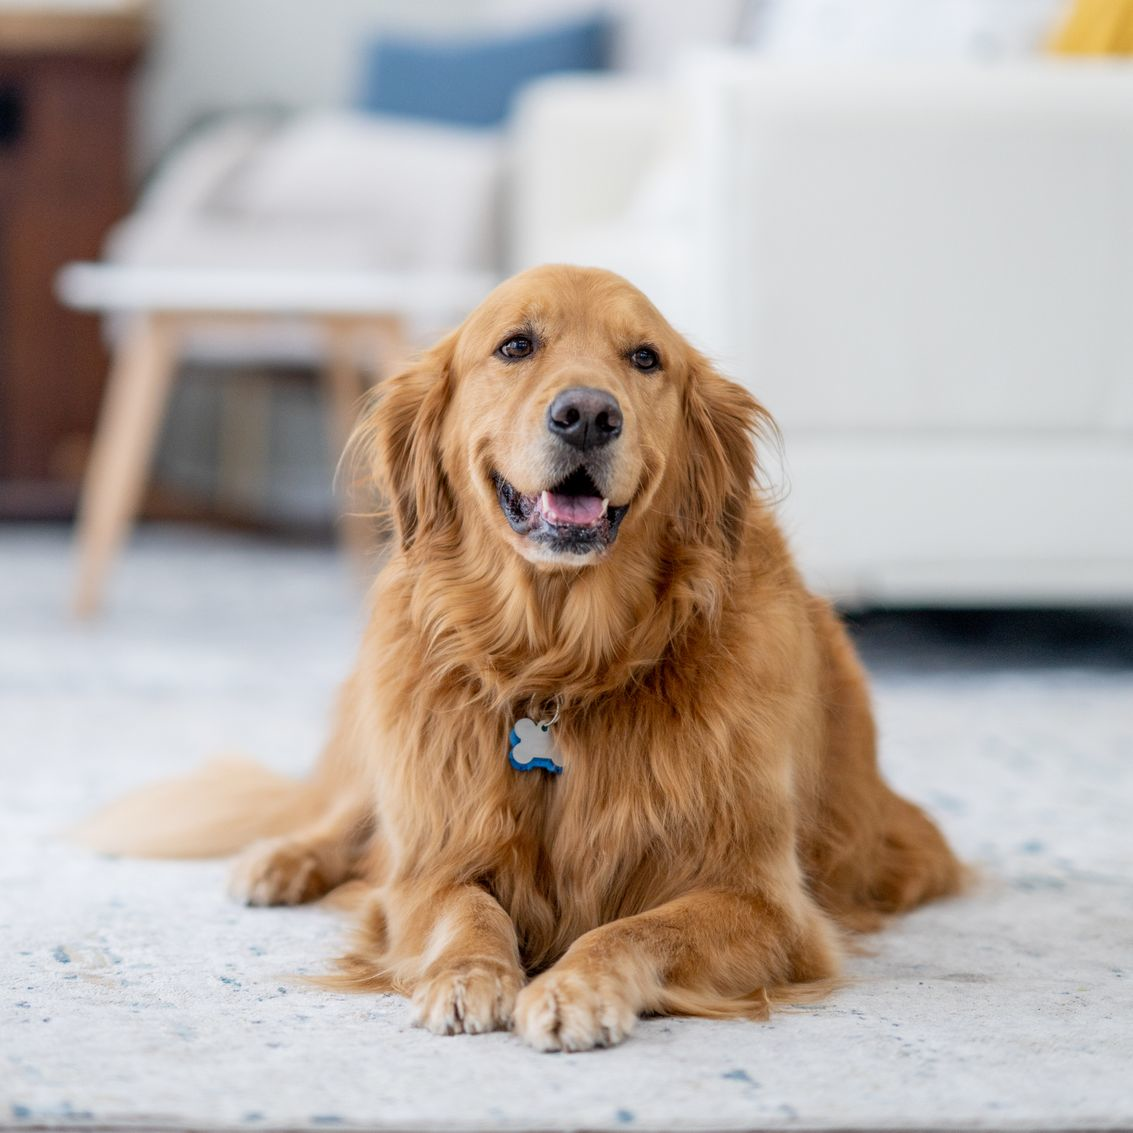
\includegraphics[width=0.5\textwidth]{figs/Dog.png}
    \caption{A nice dog.}
    \label{fig:dog}
\end{figure}

Dogs are naturally social animals, and one of their most important needs is consistent attention from their human companions. Unlike more independent pets, dogs thrive on interaction, whether it’s through play, training, exercise, or simply being near their favorite people. Many breeds, especially working and herding dogs like border collies, German shepherds, and retrievers, were bred to stay close to humans and assist with tasks, so their bond is deeply ingrained. Without enough attention, dogs can become bored, anxious, or even destructive, chewing furniture, digging, or barking excessively to release pent-up energy. Regular walks, games of fetch, and simple activities like belly rubs or grooming sessions are all ways to give them the connection they crave.

The amount of attention a dog needs can vary based on breed, age, and personality, but all dogs require daily interaction to stay happy and healthy. Puppies, for example, need lots of mental stimulation and reassurance as they learn about the world, while older dogs might be content with gentler play and companionship. Even independent breeds still want to know they’re part of the family pack. Dogs don’t just seek physical activity — they also need emotional closeness, thriving when they feel included in daily life. Whether it’s following you from room to room, curling up at your feet, or wagging their tail the second you walk through the door, their need for attention is really their way of saying, “You’re my world.” Giving them time and affection isn’t just a responsibility — it’s what makes the bond between humans and dogs so strong and rewarding.




%%%%%%%%%%%%
%%% Add fig reference to text
A nice dog can be seen in Figure~\ref{fig:dog}. This is not my dog, I have no idea who this dog belongs to. As dogs go, this a pretty cute looking dog (if you like that kind of thing).




%%%%%%%%%%
%%%%% Put a cat section FIRST

\section{Cats}
Cats are independent, curious, and graceful animals that have been cherished as companions for thousands of years. Known for their playful yet mysterious nature, they are skilled hunters with sharp reflexes and keen senses. Domestic cats come in a variety of breeds, colors, and personalities, making them adaptable to many types of households. They communicate through body language, purring, meowing, and subtle behaviors, often forming strong bonds with their owners while still valuing their independence. Cats are also known for their cleanliness, frequently grooming themselves, and they can bring comfort, companionship, and a sense of calm to those who care for them.

Cats are like tiny, furry masterminds running secret operations right under our noses. One moment, they’re curled up in a sunbeam looking like innocent little angels, and the next, they’re knocking your glass of water off the counter just to remind you who’s in charge. Their hobbies include staring at walls like they’re seeing ghosts, sprinting full speed through the house at 3 a.m. for absolutely no reason, and sitting on the exact thing you’re trying to read or type on. It’s like they have a sixth sense for the most inconvenient place to nap. And let’s not forget their dramatic flair — act like you’re ignoring them, and suddenly you’ve committed a terrible crime. Somehow, despite their sass and mischief, cats manage to convince us to feed them, clean up after them, and worship them like the royalty they clearly believe they are. Check out Tyson in Figure~\ref{fig:cat}.


\begin{figure}[h]
    \centering
    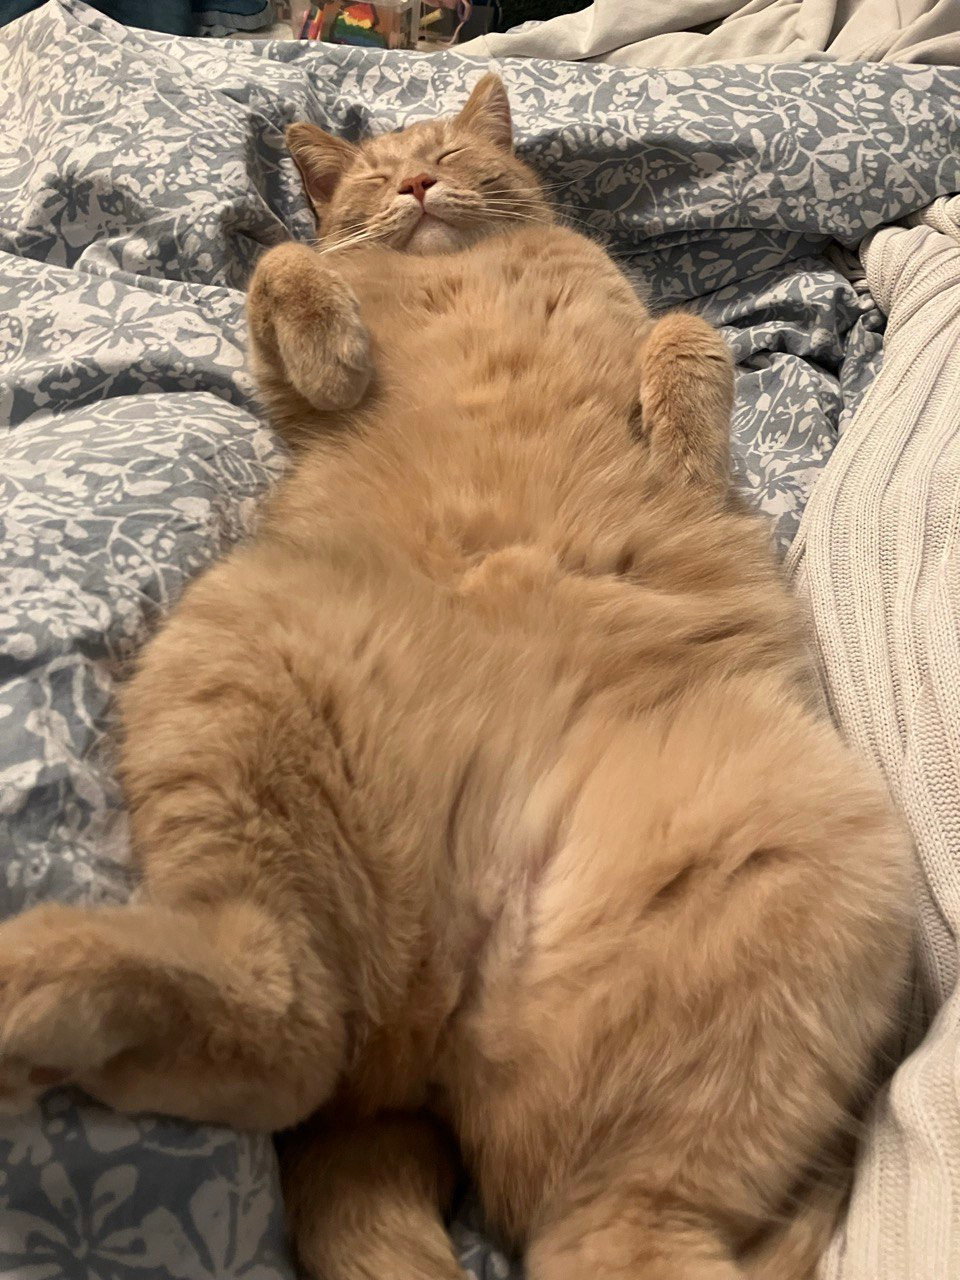
\includegraphics[width=0.5\textwidth]{figs/Cat.png}
    \caption{My cat Tyson.}
    \label{fig:cat}
\end{figure}

Cats are professional nappers, often snoozing anywhere from 12 to 16 hours a day, and sometimes even more if they’re feeling especially lazy. Their sleep is split between light dozing and deep slumber, allowing them to recharge while still being alert to sudden sounds or movements. You’ll often see them curl tightly into little fur balls, conserving heat and looking impossibly cozy, or stretch out dramatically across the couch like they own the entire living room. The way cats choose their sleeping spots is an art form in itself — sunny windowsills, freshly folded laundry, cardboard boxes, or even the exact center of your bed are all prime real estate. Their knack for turning the most inconvenient places into nap zones is part of their charm and mischief.

What’s fascinating is that cats don’t just sleep for the sake of being lazy; their snoozing habits are tied to their wild ancestors, who needed to conserve energy for bursts of hunting. Even house cats, with meals served daily in bowls, still maintain this natural rhythm of rest and sudden play. Watch closely, and you’ll notice their little paws twitch, whiskers flicker, and tails swish during dreams — a sure sign they’re chasing imaginary mice or scaling dreamland furniture. Cats seem to treat sleep as both a necessity and a hobby, perfecting the balance of ultimate relaxation and readiness. It’s no wonder we often look at them mid-nap, draped elegantly over a chair, and feel a little envious of just how good they are at doing absolutely nothing in the most graceful way possible.





%%%%%
%%%%% Add bullet points to Cats

Reasons why my cat is great:

\begin{itemize}
    \item He does not crap in the house.
        \begin{itemize}
            \item{This is the main reason}
        \end{itemize}
    \item He's furry.
    \item He is chill.
\end{itemize}

Cats have long been admired for their elegance, independence, and mysterious charm, which makes them some of the coolest animals around. \emph{They move with an effortless grace}, whether they’re leaping to the top of a bookshelf or curling up in the perfect sunbeam, and their playful yet aloof personalities have fascinated humans for centuries. Part of what makes cats so cool is their balance of affection and independence — they can be loving companions one moment and self-reliant adventurers the next. This unique mix of traits has inspired countless sayings and idioms, including the quirky phrase \textbf{“the cat’s pajamas.”} This expression dates back to the 1920s Jazz Age, when flappers and socialites embraced fun, offbeat slang to describe something or someone stylish, impressive, or top-notch. At the time, pajamas were considered trendy and a bit daring, and combining them with the ever-sophisticated cat created a phrase that perfectly captured the spirit of coolness and excellence. Today, when someone says something is “the cat’s pajamas,” they’re carrying forward a century-old tradition of celebrating whatever is truly remarkable — much like cats themselves.

Cats are like tiny, furry masterminds running secret operations right under our noses. One moment, they’re curled up in a sunbeam looking like innocent little angels, and the next, they’re knocking your glass of water off the counter just to remind you who’s in charge. Their hobbies include staring at walls like they’re seeing ghosts, sprinting full speed through the house at 3 a.m. for absolutely no reason, and sitting on the exact thing you’re trying to read or type on. It’s like they have a sixth sense for the most inconvenient place to nap. And let’s not forget their dramatic flair — act like you’re ignoring them, and suddenly you’ve committed a terrible crime. Somehow, despite their sass and mischief, cats manage to convince us to feed them, clean up after them, and worship them like the royalty they clearly believe they are.





%%%%%
%%%%% Add enumerate to Dogs.
Reasons why I’m not keen on dogs:

\begin{enumerate}
    \item They are too needy
    \item They need walking
    \item Picking up their poo
\end{enumerate}




%%%%%
%%%%% An an equation to the dogs section

The cuteness of dogs can be given by Equation~\ref{eq:einstein}

\begin{equation}
R_{\mu\nu} - \frac{1}{2} g_{\mu\nu} R + \Lambda g_{\mu\nu} = \frac{8 \pi G}{c^4} T_{\mu\nu}
\label{eq:einstein}
\end{equation}



%%%%
%%%% Add section with a table

\section{Quantifying which is best}

Using a highly scientific method, we determined which is better by doing a survey ($n=2$). These rock-solid results can be seen in Table~\ref{tab:cute}. There might be evidence that participant 1 is slightly biased towards their own cat.


\begin{table}[h]
\centering
\begin{tabular}{|c|c|c|}
\hline
Person & Cat & Dog \\
\hline
Shamit & 10 & 0 \\ 
Tina & 10 & 7 \\
\hline
\end{tabular}
\caption{Cuteness scores}
\label{tab:cute} % <--- Label goes AFTER the caption
\end{table}



%%%%%
%%% Add a biblography

%Link in paperpile
This study was done by~\cite{Legetth2021-nh,May2013-bu}.

\bibliographystyle{unsrt}
\bibliography{paperpile}  




%%%%%
%%Add natbib
\usepackage{natbib} % add this at the top
\bibliographystyle{unsrtnat}


This study was done by~\citep{Legetth2021-nh,May2013-bu}.

%%%%%
%%%Alter the margin sizes
\usepackage[top=2cm, bottom=2cm, left=2cm, right=2cm]{geometry}



%%%
%%Change font size and paper size
\documentclass[11pt,a4paper]{article}


%%%%%%
%%% Change to Times New Roman
\usepackage{mathptmx} %% add this at the top

%%%%%%%%
%%%%% Report format

\documentclass[11pt,a4paper]{report}


%%%%%
%%% Add chapters

\chapter{All about cats}
\chapter{All about Dogs}


%%%%%
%%% Add TOC

\tableofcontents



%%%%
%%%%Figure wrap

\usepackage{wrapfig} %%%% add this package at the top.

\begin{wrapfigure}[13]{r}{0.40\textwidth}
      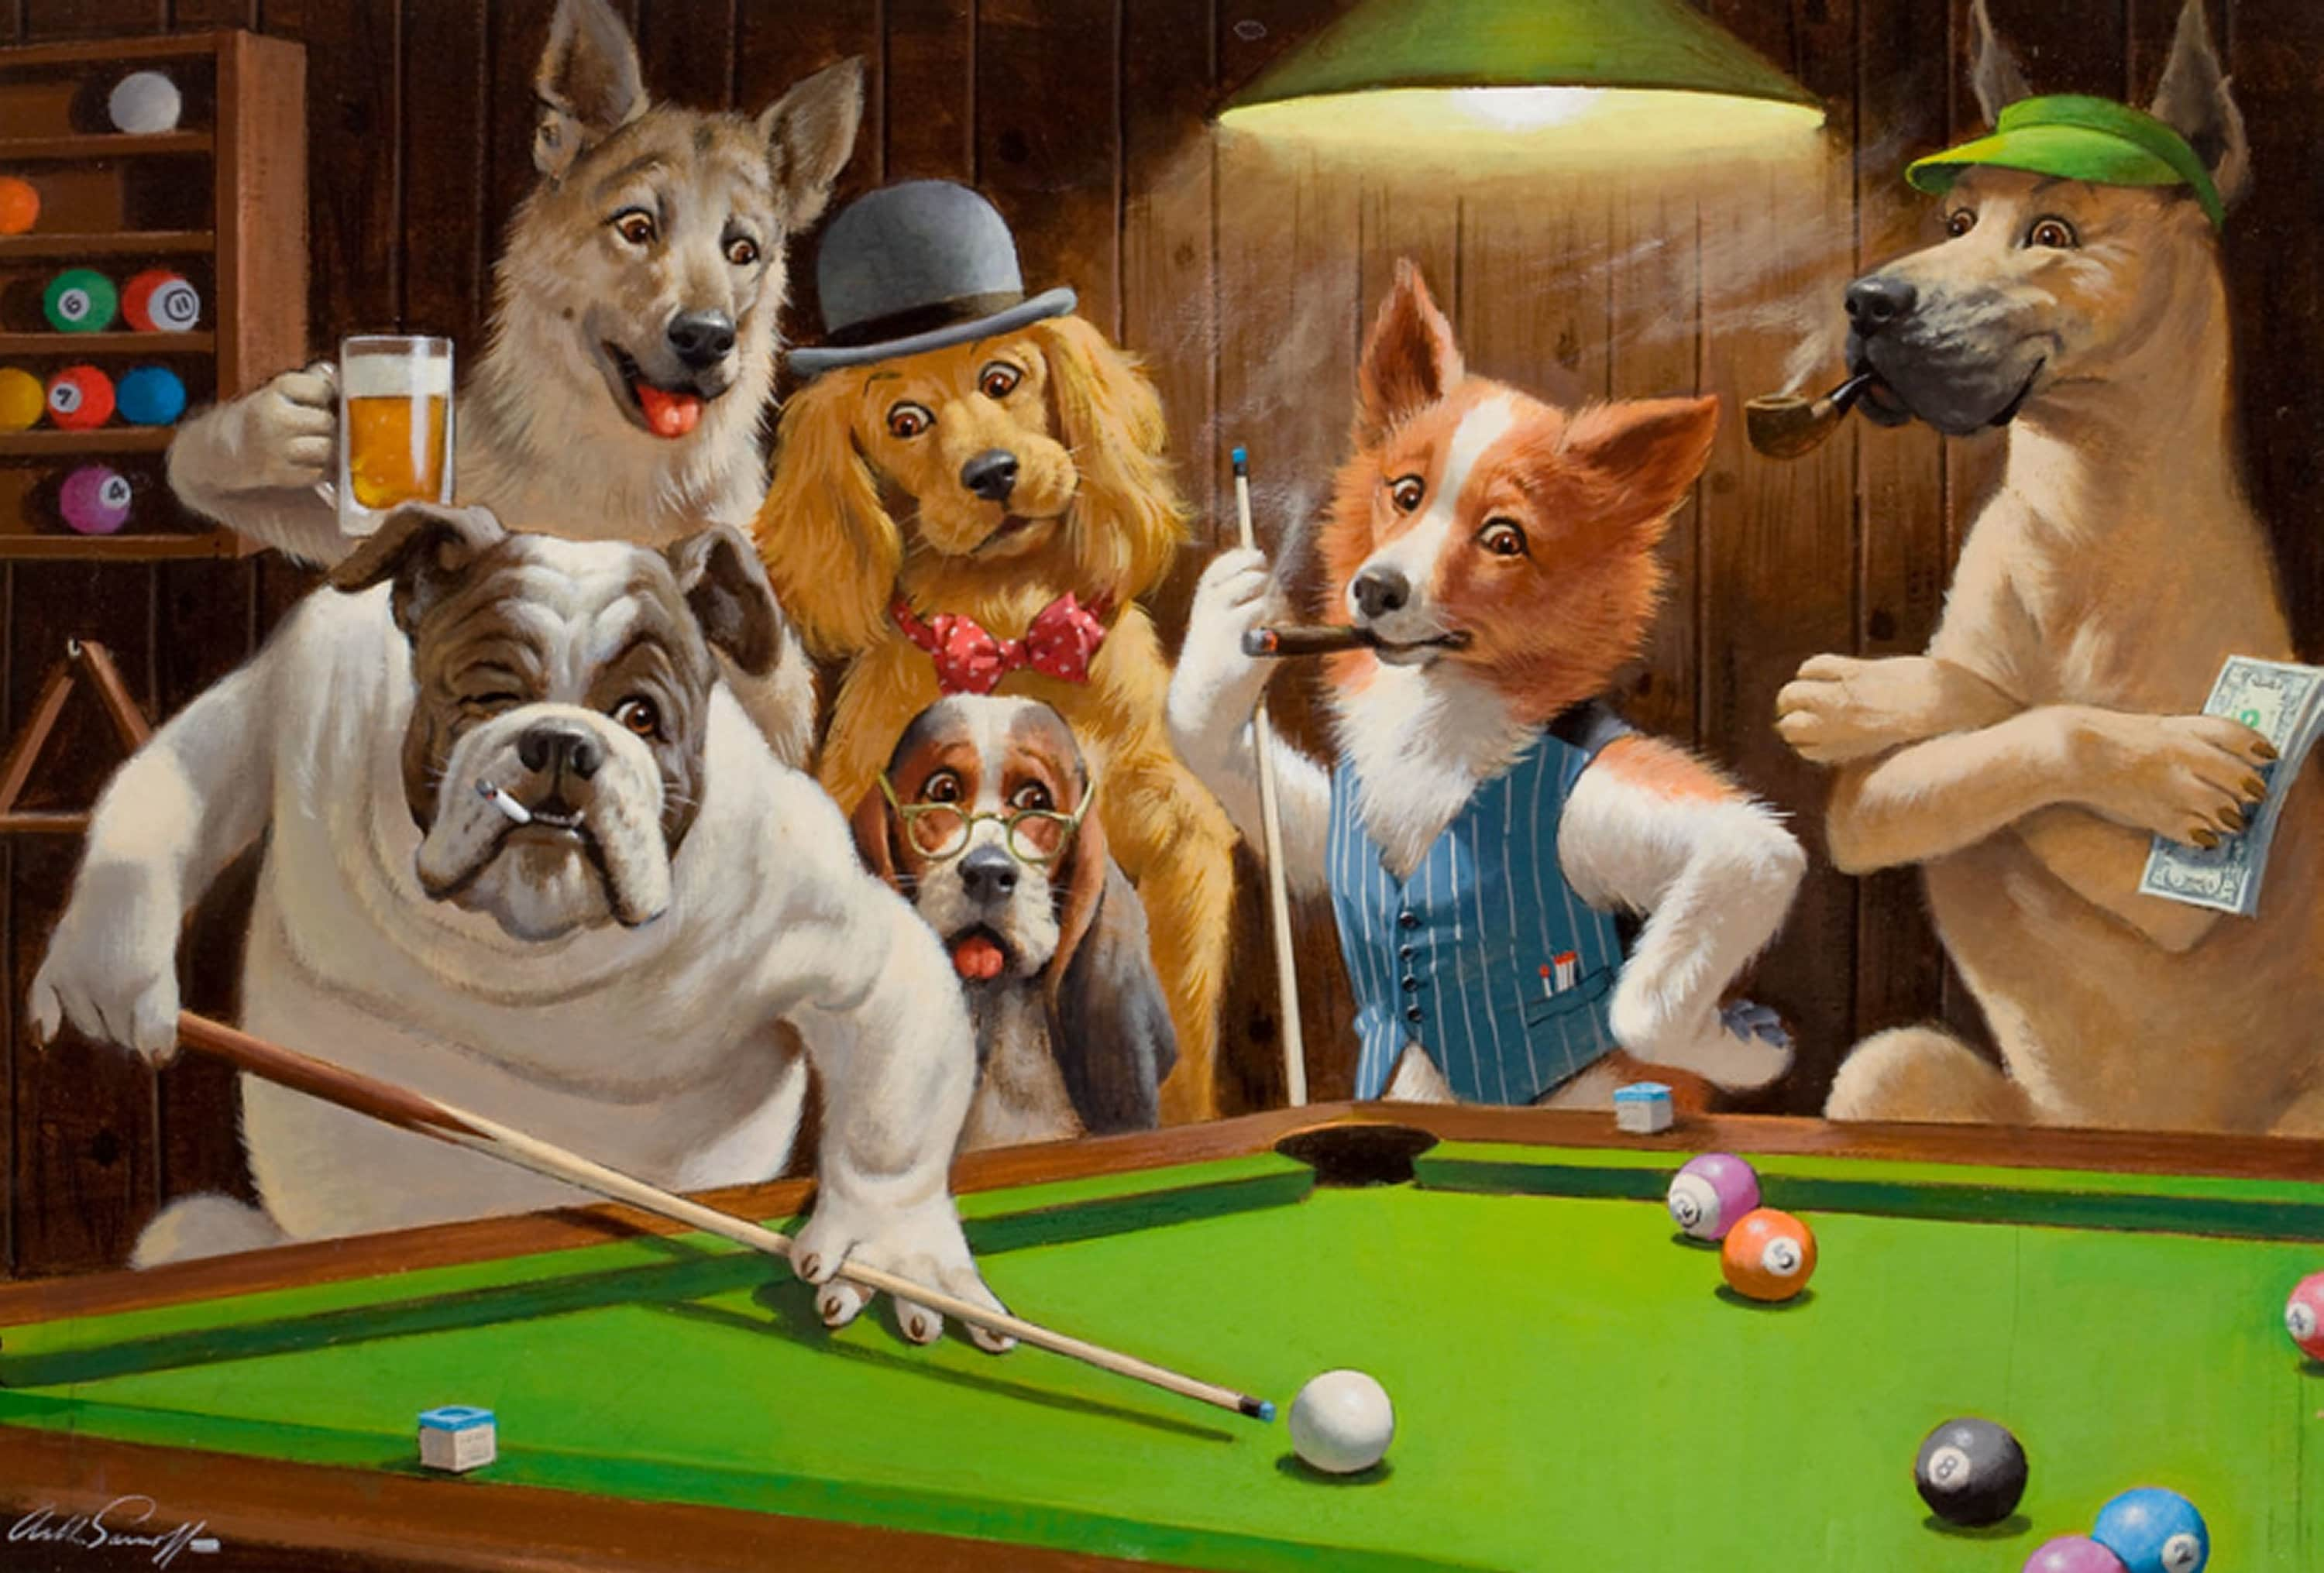
\includegraphics[width=\linewidth]{figs/dogs_pool.jpg}
      \caption{Some cool dogs shooting pool}
      \label{fig:pool}
\end{wrapfigure}


Imagine how incredible it would be if dogs could play pool — a whole new level of entertainment that combines skill, fun, and just the right amount of chaos~\ref{fig:pool}. Picture walking into a lively game room and seeing a group of dogs gathered around a pool table, each one taking turns like pros. A golden retriever carefully lines up a shot, tail wagging furiously as it nudges the cue stick with its nose, while a clever border collie studies the table intently, calculating angles like a true strategist. In the background, a bulldog might be more interested in guarding the balls, ensuring none go missing, while a mischievous terrier sneaks in a cheeky paw swipe to knock the eight ball closer to the pocket. The atmosphere would be electric — filled with excited barking, wagging tails, and the clack of billiard balls echoing through the room.

Beyond just being hilarious to watch, dogs playing pool could become a fun and unique way to bond with them. Owners could train their dogs to recognize different balls by color or pattern, rewarding them with treats for making a clean shot or setting up a clever play. It would also be a great mental workout for the dogs, challenging their problem-solving skills and keeping them engaged. Imagine doggy pool tournaments, complete with scoreboards, cheering crowds, and perhaps even a canine referee wearing a little striped shirt to keep the game fair. This could even evolve into a community event where humans and dogs team up, forming unbeatable duos where strategy and instinct merge into pure entertainment.

On top of all that, think about the joy and laughter it would bring to people watching. Videos of these talented pups would go viral instantly, spreading smiles around the world and inspiring others to try teaching their pets new tricks. Dog-friendly billiard halls could become a reality, with special tables designed for shorter players and reinforced pockets to withstand enthusiastic paws. In the end, the idea of dogs playing pool isn’t just adorable — it represents the incredible possibilities of what can happen when humans and their furry friends share fun, creativity, and a love of games. It would transform a simple pastime into an unforgettable experience, proving once again that life is always better when dogs are involved.

\usepackage{wrapfig}

%%%%
%%%%Change the colour of text

\usepackage{xcolor} % add this at the top
 
\textcolor{red}{better when dogs are involved}.

%%%%%%
%%% 1.5 spacing

\usepackage{setspace} % add this at the top
\onehalfspacing

%%%%%%
%%% shortcuts

\newcommand{\tb}{\textit{M. tuberculosis}}

Dogs can also get \tb, so keep an eye on that.

%%%%%
%%% Add a header

\usepackage{fancyhdr} % add this at the top
\pagestyle{fancy}

\fancyhead[L]{S.Soneji}
\fancyhead[R]{Cats and Dogs}



%%%%%%
%% two columns
\documentclass[11pt,a4paper,twocolumn]{report}


%%%%%%
%% Github integration







